% Diese Zeile bitte -nicht- aendern.
\documentclass[course=erap]{aspdoc}
\usepackage{tabularx}
\usepackage{multirow}
\usepackage{float}
\usepackage{xcolor}
\usepackage{pgfplots}
\usepackage{tikz}
\usepackage{wrapfig}
\usepackage{verbatim}
\usepackage[figurename=Abb.,font=small,justification=raggedright]{caption}
\definecolor{bblue}{HTML}{4F81BD}
\definecolor{rred}{HTML}{C0504D}
\definecolor{ggreen}{HTML}{9BBB59}
\definecolor{ppurple}{HTML}{9F4C7C}
\definecolor{gray1}{RGB}{50,50,50}
\pgfplotsset{compat=1.5}
\graphicspath{ {./res/} }
\renewcommand{\arraystretch}{1.1}
\newcommand{\hexdump}[2]{
  % #1 = temp file name       
  % #2 = input file name
 \begin{figure}[H]
   \small
   \verbatiminput{#1}
   \vspace*{-5mm}
   \caption{#2}
%   \label{fig:#4}
 \end{figure}
}

\newcommand{\verbatimdump}[1]{
  % #1 = temp file name       
  % #2 = input file name
 \begin{figure}[H]
   \small
   \verbatiminput{#1}
   \vspace*{-5mm}
 \end{figure}
}

\newcommand{\imagewrap}[5]{
 \begin{wrapfigure}{#3}{#5}
  \vspace*{-5mm}
    \centering
   \includegraphics[width=#4]{#1}
   \caption{#2}
 \end{wrapfigure}
}

\newcommand{\image}[3]{
 \begin{figure}[H]
   \includegraphics[width=#3]{#1}
 \centering
   \caption{#2}
 \end{figure}
}

%%%%%%%%%%%%%%%%%%%%%%%%%%%%%%%%%
%% TODO: Ersetzen Sie in den folgenden Zeilen die entsprechenden -Texte-
%% mit den richtigen Werten.
\newcommand{\theGroup}{121} % Beispiel: 42
\newcommand{\theNumber}{A203} % Beispiel: A123
\author{Adam Karamelo \and Philipp Czernitzki}
\date{Wintersemester 2021/22} % Beispiel: Wintersemester 2019/20
%%%%%%%%%%%%%%%%%%%%%%%%%%%%%%%%%

% Diese Zeile bitte -nicht- aendern.
\title{Gruppe \theGroup{} -- Abgabe zu Aufgabe \theNumber}

\begin{document}
\maketitle

\section{Einleitung}
\imagewrap{example.png}{Rastergrafik 5x5}{r}{0.20\textwidth}{0.25\textwidth}
Für die Darstellung von Grafiken auf digitalen Bildschirmen existieren eine Vielzahl von Bildformaten. Das Bitmap Format von Microsoft, kurz \textbf{BMP Format}, war ein beliebtes Format um Rastergrafiken darzustellen.  Diese Grafiken können jedoch unkomprimiert Unmengen an Speicherplatz verbrauchen, weshalb es hilfreich ist diese zu komprimieren. Über die \textbf{Lauflängenkodierung} können Pixel gleicher Farbwerte zusammengefasst werden und so die Dateigröße minimiert werden. Formate wie PNG und JPEG, die standardmäßig komprimiert sind, erfreuen sich heute großer Beliebtheit. Diese Arbeit beschäftigt sich mit der \textbf{Komprimierung von Bilddateien} im Bitmap Format durch die Lauflängenkodierung. Anhand eines Beispielbildes wird das Bitmap Format und die Komprimierung über die Lauflängenkodierung erläutert. Es wird ein Algorithmus für die Kompression erarbeitet und seine Funktionsweise, Performanz und Korrektheit analysiert und geprüft.



\section{Lösungsansatz}

\subsection{Bitmap Format}
8 Bits per Pixel Bitmaps~\cite{aboutBitmaps} bestehen aus vier Komponenten, einem \textbf{BitmapFileHeader}~\cite{bitmapFileHeader}, einem \textbf{Bitmap Information Header}~\cite{bitmapHeaderTypes}, einer \textbf{Color Palette}, und einem oder mehreren \textbf{Pixelindizes}. Die Color Palette enthält  alle darstellbaren Farben der Grafik im RGB-Format, d.h. in \textbf{\textcolor{blue}{blau}}, \textbf{\textcolor{green}{grün}} und \textbf{\textcolor{red}{rot}}. Jeder Pixelindex zeigt auf einen RGB-Eintrag in der Color Palette wodurch der Farbwert des Pixels erhalten wird. Im folgenden wird von 8 Bits per Pixel Bitmaps ausgegangen, für andere Werte kann sich das Format ändern.

\subsubsection{Bitmap File Header}
Der BitmapFileHeader~\cite{bitmapFileHeader} gibt den Typ, die Dateigröße und das Offset zu den Pixelindizes der Bitmap an. Er ist 14 Bytes groß.

\hexdump{res/example_28_5x5_fileheader.txt}{BitmapFileHeader für Rastergrafik}
\begin{table}[h!]
\begin{tabular}{ |p{6em}|p{3em}|p{25.75em}| }
    \hline
    \textbf{Feld} & \textbf{Bytes} & \textbf{Beschreibung} \\
    \hline
    Type & 2 & Zeigt, dass es sich um eine Bitmap handelt.\newline Muss auf \textbf{0x4d42} gesetzt sein. \\ \hline
    Size & 4 & Die Dateigröße in Bytes \\
    \hline
    Reserved1 & 2 & Verwendet von Bildverarbeitungsprogrammen,\newline normalerweise mit \textbf{`0'} initialisiert. \\
    \hline
    Reserved2 & 2 & Verwendet von Bildverarbeitungsprogrammen,\newline normalerweise mit \textbf{`0'} initialisiert. \\
    \hline
    OffBits & 4 & Offset in Bytes von Anfang der Datei bis zu den Pixelindizes. \\
    \hline
\end{tabular}
\caption{Felder des BitmapFileHeader}
\end{table}



\subsubsection{Bitmap Information Header}
Im Information Header stehen Informationen über das Bild der Bitmap. \newline Unter anderem ist die Breite, die Höhe, die verwendete Kompression und die Größe der Pixelindizes in Bytes enthalten.\newline
% \subsubsection{BitmapInfoHeader}

% Der BitmapV4Header und BitmapV5Header erweitern jeweils den BitmapInfoHeader.

\begin{table}[h!]
\begin{tabular}{ |p{6em}|p{3em}|p{25.75em}|  }
    \hline
    \textbf{Feld} & \textbf{Bytes} & \textbf{Beschreibung} \\
    \hline
    Size & 4 & Die Anzahl an Bytes benötigt \\
    \hline
    Breite & 4 & Die Breite in Pixel \\
    \hline
    Höhe & 4 & Die Höhe in Pixel \\
    \hline
    Planes & 2 & Anzahl an Flächen, muss \textbf{`1'} betragen. \\
    \hline
    BitCount & 2 & Anzahl an Bits die einen Pixel definieren \\
    \hline
    Compression & 4 & \textbf{`0'} - keine Komprimierung\newline \textbf{`1'} - 8bpp Lauflängenkodierung \\
    \hline
    SizeImage & 4 & Größe der komprimierten Pixeldaten in Bytes. \newline Wenn \textbf{`0'} dann hat keine Komprimierung stattgefunden. \\
    \hline
    XPelsPerMeter & 4 & Horizontale Auflösung in Pixel pro Meter des Zielgerätes. \newline Wenn \textbf{`0'} dann keine Präferenz \\
    \hline
    YPelsPerMeter & 4 & Vertikale Auflösung in Pixel pro Meter des Zielgerätes. \newline Wenn \textbf{`0'} dann keine Präferenz \\
    \hline
    ClrUsed & 4 & Anzahl an Farbindizes. Wenn \textbf{`0'} dann nutzt die Bitmap \textbf{2\textasciicircum bitCount} Einträge aus der Color Palette \\
    \hline
    ClrImportant & 4 & Anzahl an Farbindizes erforderlich um die Bitmap anzuzeigen. Wenn \textbf{`0'} dann sind alle Farbindizes erforderlich. \\
    \hline
\end{tabular}
\caption{Felder des BitmapInfoHeader}
\end{table}

Das Bitmap Format spezifiziert verschiedene Information Header in unterschiedlichen Größen. Die umgesetzte Implementierung beschränkt sich explizit nur auf die von Microsoft dokumentierten Information Header: \textbf{BitmapCoreHeader}~\cite{bitmapCoreHeader} (12 Bytes), \textbf{BitmapInfoHeader}~\cite{bitmapInfoHeader} (40 Bytes), \textbf{BitmapV4Header}~\cite{bitmapV4Header} (108 Bytes) und \textbf{BitmapV5Header}~\cite{bitmapV5Header} (124 Bytes). Andere Versionen des Information Header sind nicht dokumentiert oder wurden von Dritten entwickelt. BitmapV4Header und BitmapV5Header erweitern die Felder des in Tabelle 2 gezeigten BitmapInfoHeader.

\hexdump{res/example_28_5x5_infoheader.txt}{BitmapInfoHeader für Rastergrafik}

\subsubsection{Sonderfall: BitmapCoreHeader}
Der BitmapCoreHeader~\cite{bitmapCoreHeader} unterscheidet sich vom BitmapInfoHeader, BitmapV4Header und BitmapV5Header. Die \textit{Höhe und Breite des Headers werden \textbf{in 2-Byte} statt den üblichen 4-Byte} angegeben. Desweiteren spezifiziert er \textit{kein Feld für die Komprimierung}, daher kann eine Bitmap mit einem BitmapCoreHeader nicht komprimiert werden. Ebenfalls sind \textit{Einträge in der Color Palette \textbf{in 3-Byte} statt 4-Byte} angegeben.
\newline 
Die Implementierung wandelt einen BitmapCoreHeader dementsprechend in einen BitmapInfoHeader um, welcher die Komprimierung durch die Lauflängenkodierung unterstüzt.
\newline

\begin{table}[h!]
\begin{tabular}{ |p{6em}|p{3em}|p{25.75em}|  }
    \hline
    \textbf{Feld} & \textbf{Bytes} & \textbf{Beschreibung} \\
    \hline
    Size & 4 & Zeigt, dass es sich um eine Bitmap handelt.\newline Muss auf \textbf{0x4d42} gesetzt sein. \\ \hline
    Width & 2 & Breite der Bitmap in Pixel \\
    \hline
    Height & 2 & Höhe der Bitmap in Pixel \\
    \hline
    Planes & 2 & Anzahl an Flächen, muss \textbf{`1'} betragen. \\
    \hline
    BitCount & 2 & Anzahl an Bits per Pixel \\
    \hline
\end{tabular}
\caption{Felder des BitmapCoreHeader}
\end{table}

\hexdump{res/example_0C_5x5_infoheader.txt}{BitmapCoreHeader für Rastergrafik}

\subsubsection{Color Palette}
Die Farbpalette der Bitmap besteht aus mehreren \textbf{RGBQuad}~\cite{rgbQuad} (4-Tupel) oder \textbf{RGBTriple}~\cite{rgbTriple} (3-Tupel) Einträgen. Alle Farbwerte liegen im Intervall von [0, 255]. Es ist zu beachten, dass nur der BitmapCoreHeader RGBTriple nutzt, alle anderen unterstützten Header nutzen RGBQuad.
\newline
\begin{itemize}
  \item \textbf{RGBQuad}:
  
  (\textbf{\textcolor{blue}{blau}}, \textbf{\textcolor{green}{grün}}, \textbf{\textcolor{red}{rot}}, \textbf{reserviert} = 0) \newline
  Das reservierte Byte soll 0 sein
  \item \textbf{RGBTriple}: (\textbf{\textcolor{blue}{blau}}, \textbf{\textcolor{green}{grün}}, \textbf{\textcolor{red}{rot}})
  
\end{itemize}
Die maximale Größe der Color Palette ergibt sich aus dem \textbf{bitCount} Feld des Information Headers über \textbf{2\textasciicircum bitCount}. Eine 8 Bit per Pixel Bitmap kann maximal 256 Einträge besitzen.

\hexdump{res/example_28_5x5_colorpalette.txt}{Color Palette der Rastergrafik}

\subsubsection{Pixelindizes / Pixeldaten}
Pixeldaten werden über Indizes auf die Color Palette spezifiert.
Ein Pixelindex ist \textbf{bitCount} groß. Gemäß Aufgabenstellung werden \textbf{8 Bits per Pixel} betrachtet. Entsprechend ist $ bitCount = 8 $. Ein Pixelindex kann Werte im Intervall von [0, 255] annehmen.
Pixelindizes stehen zeilenweise nebeneinander. Jede Zeile, auch \textbf{Scan Line} genannt, ist 4-Byte aligned und wird am Ende falls nötig mit \textbf{Padding Bytes (0x00)} gefüllt. Die Beispiel Rastergrafik (5x5 Pixel) enthält 3 Padding Bytes (0x00) am Ende jeder Scan Line. Der erste Pixelindex beschreibt den Pixel links unten im Bild, da Bitmaps von unten nach oben konstruiert werden.~\cite{medium}

\hexdump{res/example_28_5x5_pixeldata.txt}{Pixelindizes der Rastergrafik}
In der Abbildung ist zu erkennen, dass 5 gleiche (blaue) Pixel geschrieben werden und 3 Padding Bytes folgen.

\subsection{Implementierung}
Ziel der Implementierung ist es eine Bitmap über die Lauflängenkodierung (run-length-encoding) zu komprimieren.

\subsubsection{Annahmen}
\begin{itemize}
  \item Das Programm muss gemäß Aufgabenstellung explizit nur 8 Bit per Pixel Bitmaps unterstützen.
  \item Color Profiles wie sie im BitmapV5Header existieren können, werden nicht unterstützt.
  \item Die Komprimierung unterstützt Bilder bis zur einer Auflösung von 7680x7680. Das heißt Bilder mit einer Auflösung bis zu 8K werden unterstützt. \newline\newline
  \textit{Die theoretisch maximalste Auflösung beträgt 2.147.483.648 Pixel.
  Da die komprimierten Pixelindizes in einen Buffer geschrieben werden, der mit \textbf{malloc(size\_t)} alloziiert wird, hängt die maximal darstellbare Auflösung von der maximalen Größe der alloziierbaren Bytes ab. Auf einem 32 Bit System können bis zu 4.294.967.296 Bytes alloziiert werden. Im schlimmsten Fall sind alle nebeneinanderliegende Pixelindizes unterschiedlich und wir schreiben nur im \hyperref[sec:Encoded]{Encoded Modus}. Dann werden für jeden Pixelindex immer 2-Byte geschrieben.}

\end{itemize}

\subsubsection{Validierung}
Bevor die Bitmap komprimiert wird, prüft die Implementierung die Header Felder aus der Spezifikation, ob diese valide und richtig für eine unkomprimierte Bitmap gesetzt sind.
\subsubsection{Komprimierung}
Es wird das \textbf{Compression} Feld im Bitmap Information Header auf \textbf{`1'} gesetzt. Das Bitmap Format bietet 2 Modi für das schreiben von komprimierten Pixelindizes.
\paragraph{Encoded Modus}
\label{sec:Encoded}
Im Encoded Modus werden gleiche nebeneinander stehende Pixelindizes zusammengefasst.
Man schreibt die Wiederholungen und den Pixelindex. Das heißt es werden 2-Byte in folgendem Format geschrieben: \textbf{\textit{<Wiederholungen> <Pixelindex>}}
In der Beispielrastergrafik befinden sich in der ersten Scan Line \textbf{5 gleiche Pixel}, dargestellt als \textbf{\textit{0x00 0x00 0x00 0x00 0x00}}, diese werden entsprechend zu \textbf{\textit{0x05 0x00}} zusammengefasst.

\paragraph{Absolute Modus}
Im Absolute Modus werden unterschiedliche nebeneinander stehende Pixelindizes zusammengefasst. Man schreibt ein Nullbyte, die Anzahl der unterschiedlichen Pixelindizes und dann die Pixelindizes. Das Format sieht wie folgt aus:\newline
\textbf{\textit{<Nullbyte> <Anzahl> <1.Pixelindex> <2. Pixelindex> <3.PixelIndex> ...}}\newline
Dieser Modus ist 2-Byte aligned, das heißt es muss gegebenfalls noch ein Nullbyte zum Schluss geschrieben werden, sodass die Menge der geschriebenen Bytes gerade bleibt. Ebenfalls muss beachtet werden, dass die Anzahl mindestends drei beträgt, damit dieser Modus verwendet werden kann.

\paragraph{Scan Line Ende}
Ist eine Scan Line durch den Absolute und/oder Encoded Modus komprimiert, werden zwei weitere Bytes geschrieben. Im Normalfall schreibt man am Ende einer Zeile \textbf{\textit{0x00 0x00}}, um das Zeilenende zu kennzeichnen. Falls man sich in der letzten Scan Line befindet wird jedoch \textbf{\textit{0x00 0x01}} geschrieben, um das Ende der Bitmap zu kennzeichnen.

\subsubsection{Optimierung der Kompressionsrate}
\label{sec:Optimierung}
Die Kompressionsrate kann erhöht werden, wenn man den Encoded Modus nur verwendet wenn nötig. Sind mindestens drei nebeneinanderliegende Pixel gleich oder der Absolute Modus kann nicht verwendet werden weil die Anzahl kleiner gleich zwei beträgt, soll der Encoded Modus verwendet werden. In allen anderen Fällen soll der Absolute Modus verwendet werden. Sind zwei nebeneinanderliegende Pixel gleich soll der Absolute Modus verwendet werden.
\newline
\newline
\textbf{Pixelindizes}
\vspace*{-2mm}
\verbatiminput{res/optimization.txt}
\textbf{Komprimiert ohne Optimierung} - 2 gleiche Pixel in Encoded Modus
\vspace*{-2mm}
\verbatiminput{res/optimization_without.txt}
\textbf{Komprimiert mit Optimierung}
\vspace*{-2mm}
\verbatiminput{res/optimization_with.txt}


Die Implementierungen von Version 0 bis 2 nutzen diese Optimierung.

\subsection{Implementierte Versionen}
% Vier Versionen von Lauflängekodierung sind implementiert geworden: $bmp\_rle.c$, $bmp\_rle\_V1.c$ ,$bmp\_rle\_V2.c$ und $bmp\_rle\_V3.c$. Sie werden unten beschrieben und analysiert.

\subsubsection{RLE Encoded Modus V3 (\textit{bmp\_rle\_encode\_V3.c})}
Die Version 3 ist ein naiver Ansatz der Lauflängekodierung. Sie nutzt nur den Encoded Modus der Bitmap Komprimierung. Der Algorithmus geht durch die Pixeldaten, vergleicht jeweils zwei Pixelindizes und zählt in einem Zähler wie oft der Pixelindex unverändert bleibt. Ist der nächste Pixelindex nicht mehr gleich, wird der Zähler und Pixelindex im Encoded Modus geschrieben.

\subsubsection{RLE Encoded und Absolute Modus V2 (\textit{bmp\_rle\_V2.c})}
Die Version 2 arbeitet mit 2 Zählern gleichzeitig: \textbf{reps} und \textbf{diff}. Pixel werden paarweise verglichen. Wenn sie unterschiedlich sind wird \textbf{diff} inkrementiert und \textbf{reps} zurückgesetzt. Wenn sie gleich sind, werden \textbf{reps} und \textbf{diff} beide inkrementiert. Diff wird auch inkrementiert, um den Fall zu vermeiden, dass 2 gleiche Pixel im Encoded Modus geschrieben werden, siehe \hyperref[sec:Optimierung]{hier}. Nur wenn ein unterschiedliches Pixel nach einer Reihe von mindestens 3 gleichen Pixeln entdeckt wird, werden die Pixeldaten geschrieben. Zuerst wird die \textbf{diff} Anzahl an Pixeln geschrieben. Danach werden die \textbf{reps} von Pixeln geschrieben.

\subsubsection{RLE Encoded und Absolute Modus V1 (\textit{bmp\_rle\_V1.c})}
Die Version 1 vergleicht jeden Pixel mit den nächsten zwei, um drei gleiche zu finden. So lange keine drei gleichen Pixeln gefunden werden wird der Zähler \textbf{diff} inkrementiert. Bei drei gleichen Pixel, werden die bereits gezählten \textbf{diff} geschrieben. Dann wird gezählt ob es weitere gleiche Pixel in einem Zähler \textbf{rep} gibt. Gibt es keine gleichen Pixel mehr, werden die gleichen Pixel \textbf{rep} geschrieben und es werden wieder \textbf{diff} gezählt. 

\subsubsection{RLE Encoded und Absolute Modus mit SIMD Intrinsics V0 (\textit{bmp\_rle.c})}
Bei Version 0 werden SIMD Intrinsics benutzt. SIMD ermöglicht durch Vektorisierung, Pixel in 16 Byte Blöcken zu vergleichen und zu speichern. Durch die Intrinsics Funktion $\_mm\_cmpeq\_epi8$ werden jeweils zwei nebeneinanderstehende Pixel verglichen. Eine Maske gibt an ob zwei Pixel gleich waren (0xff) oder ob diese unterschiedlich waren (0x00). Daraufhin werden unterschiedliche Pixel in einem Zähler \textbf{diff} und gleiche Pixel in einem Zähler \textbf{rep} gezählt. Je nachdem wird entschieden ob der Absolute Modus oder Encoded Modus zum Schreiben verwendet wird. Wenn wir im Absolute Modus schreiben berechnen wir wie oft wir mit SIMD 16 Byte Blöcke schreiben können und schreiben die unaligned Pixeldaten mit \textit{memcpy}.


\subsubsection{Coding Style}
Die durch die Aufgabenstellung erhaltene Methodensignatur wurde geringfügig verändert um die Naming Konvention von Variablen in camelCase zu bewahren.

\section{Korrektheit}
\imagewrap{example.png}{Rastergrafik 5x5}{r}{0.17\textwidth}{0.25\textwidth}
\vspace*{2mm}
Zunächst vergleichen wir die Rastergrafik rechts. Es ist zu erkennen, dass die Bitmap Komprimierung zwei Byte mehr verwendet wenn die Rastergrafik mit der Lauflängenkodierung komprimiert ist. Das liegt daran, dass die Rastergrafik wenig gleiche Pixel besitzt und diese nicht zusammengefassen werden. Im Absolute Modus werden mindestens sechs Bytes geschrieben und im Encoded Modus mindestens zwei Byte. 


\hexdump{res/example_28_5x5.txt}{Unkomprimierte Rastergrafik}
Kann der Algorithmus nun die Pixel nicht zusammenfassen, entspricht das einem erheblichen Mehraufwand/Verbrauch für einen 1-Byte Pixel.\newline

\hexdump{res/example_28_5x5_compressed.txt}{Komprimierte Rastergrafik 5x5 - Version 0}
\hexdump{res/example_28_5x5_compressed_V1.txt}{Komprimierte Rastergrafik 5x5 - Version 1}
\image{./res/pink_28_150x10}{Einfarbige Bitmap 150x10}{0.9\textwidth}
Eine einfarbige Bitmap hingegen in der Größe 150x10 wird mit einer Kompressionsrate von 16:1 komprimiert, dies entspricht einer um 93\% reduzierten Bitmapgröße. In diesem Fall werden bis zu 150 Pixel in einer Zeile zusammengefasst und als 2-Byte im Encoded Modus geschrieben.
\hexdump{res/pink_28_150x10_compressed.txt}{Komprimierte Einfarbige Rastergrafik 150x10 - Version 0}
\hexdump{res/pink_28_150x10_compressed_V1.txt}{Komprimierte Einfarbige Rastergrafik 150x10 - Version 1}
% \subsection{Randfälle}
% Bei allen implementierten Versionen des RLE Algorithmus, werden diese Randfälle wie folgendes behandelt werden:
% \begin{itemize}
%   \item Der Input Pointer, der die Pixeldaten des eingegebenen Bildes liest, wird nie das letzte Pixel überschreiben. Hier wird sicher gestellt, dass kein Segmentation Fault auftritt.
%   \item Die Bitmap Padding, die am Ende von jedem Scan Line erscheinen, ermöglichen immer eine 4 byte-aligned große Datei. Sie werden korrekt uberschritten, damit kein Vergleich zwischen Padding Bytes und PixelDaten passiert.
%   \item Wenn das Ende von jedem Scan line kommt oder das letzte Pixel gelesen wird, werden entschprechend die End of Line und End of File bytes geschrieben.
%   \item Die maximale Anzahl der zu schreibenden Pixel ist 255, weil das in einem Byte representierbar sein soll. Wenn die reps 255 wird sollen die gleiche Pixel geschrieben werden. Wenn diff 255 wird, muss noch sicher gestellt werden, dass die kommenden Pixeln nicht die zu schreibenden beeinflussen. Das bedeutet, wenn die letzten zwei verglichenen Pixeln gleich waren, und der kommende auch gleich ist, wird diff passend dekrementiert und geschrieben. Dies gescheht, damit die kommende Pixel zusammen in encoded Modus geschrieben werden können.
% \end{itemize}


\section{Performanzanalyse}
In diesem Abschnitt wird auf die Laufzeitanalyse und Kompressionsrate der verschiedenen Ansätze des Algorithmus eingegangen. Getestet wurde auf einem System mit einem Intel Core i5-8300H CPU, 2.30GHz, 8GB Arbeitsspeicher, WSL Ubuntu 18.04, 64 Bit, Kernel 4.4.0-19041-Microsoft. Kompiliert wurde mit GCC 7.5.0 mit der Option -O2.\newline
Wichtig zu erwähnen ist, dass die vier Implementierungsvarianten sich unterschiedlich im Bezug auf die Eingabedatei verhalten. Hier ist zwischen drei Fällen zu unterscheiden:

\begin{itemize}
  \item \textbf{Worst Case Image} Bilder, die keine drei nacheinander gleiche Pixel haben.\newline getestet mit: \textcolor{gray1}{lena\_gray\_6C\_512x512.bmp , lena\_7C\_3x10.bmp,\newline random\_0C\_10x10.bmp}
\item \textbf{Average Case Image:} Bilder die eine vernünftige Menge an gleichen und abwechselnden Pixelindizes beinhalten.\newline getestet mit: \textcolor{gray1}{lena\_7C\_512x512.bmp, deer\_7C\_397x706.bmp, nasa\_7C\_523x549.bmp,\newline nature\_7C\_380x570.bmp, people\_7C\_476x317.bmp, planet\_7C\_499x499.bmp,\newline tank\_7C\_277x182.bmp}
  \item \textbf{Best Case Image:} Bilder die nur aus einer Farbe, einem Pixelindex bestehen.\newline
  getest mit: \textcolor{gray1}{pink\_7C\_512x512.bmp}
\end{itemize}

\subsection{Laufzeitanalyse}
In Abbildung \ref{fig:Laufzeit} wird die Laufzeit der vier verschiedenen Implementierungen verglichen. Es wurden jeweils drei Bilder der Größe 512x512 (aus jeder Kategorie) getestet.\newline 
Die Version 0 (V0) ist mit SIMD Optimierungen in allen Fällen um einen Faktor 1.82 bis 4 performanter, abhängig vom Typ der Eingabedatei.\newline
V0, V1 und V2 kodieren die Pixel sowohl in Encoded als auch in Absolute Modus.\newline
Dank SIMD, werden in V0 die Pixel in 16 Byte Blöcken geladen und gespeichert. Deshalb gewinnen wir stark an Performanz.\newline Die V1 inkrementiert abwechselnd \textbf{reps} und \textbf{diff} gemäß des Resultats der zwei Pixelvergleiche, was einen Overhead erzeugt.\newline
Die V2 macht nur einen paarweisen Vergleich, das aktuellste mit dem nächsten. Allerdings arbeitet V2 mit zwei Zählern die oft zusammen inkrementiert werden und auch öfters überprüft werden müssen, was sich stark auf die Laufzeit einwirkt.
Bei häufig wechselnden Pixelwerten ist V2 performanter, sonst V1.
Die V3 ist in diesem Fall sehr ineffizient, weil nach unterschiedlichen Pixeln immer direkt geschrieben wird.

Interessant zu verstehen ist warum Worst Case Images eine bessere Laufzeit als Average Case Images haben, bei den Implementierungsversionen, die beide Modi nutzen. Denn im Worst Case wird nur ein Zähler \textbf{diff} inkrementiert, da alle Pixel unterschiedlich sind. Somit werden weniger Bedingungen überprüft.

\begin{figure}[h]
\centering
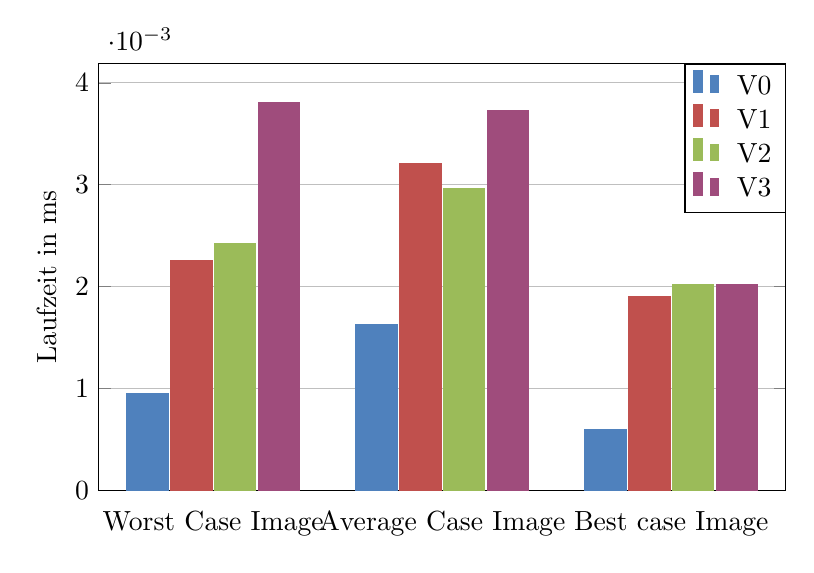
\begin{tikzpicture}
    \begin{axis}[
        width  = 0.85*\textwidth,
        height = 7cm,
        major x tick style = transparent,
        ybar=2*\pgflinewidth,
        bar width=15pt,
        ymajorgrids = true,
        ylabel = {Laufzeit in ms},
        symbolic x coords={Worst Case Image,Average Case Image,Best case Image},
        xtick = data,
        scaled y ticks = true,
        enlarge x limits=0.25,
        ymin=0,
        legend cell align=left,
        legend style={
                at={(1,1)},
                anchor=north east,
                column sep=1ex
        }
    ]
        \addplot[style={bblue,fill=bblue,mark=none}]
            coordinates {(Worst Case Image, 0.000949) (Average Case Image, 0.001626) (Best case Image,0.000599)};

        \addplot[style={rred,fill=rred,mark=none}]
             coordinates {(Worst Case Image,0.002252) (Average Case Image, 0.003207) (Best case Image,0.001905)};

        \addplot[style={ggreen,fill=ggreen,mark=none}]
             coordinates {(Worst Case Image,0.002425) (Average Case Image,0.002965) (Best case Image, 0.002021)};

        \addplot[style={ppurple,fill=ppurple,mark=none}]
             coordinates {(Worst Case Image,0.003809) (Average Case Image,0.003733) (Best case Image,0.002016)};

        \legend{V0, V1, V2, V3}
    \end{axis}
    
\end{tikzpicture}
\caption{Laufzeit von Implementierungsversionen für verschiedene Bild Typen}
\label{fig:Laufzeit}
\end{figure}

\subsection{Kompressionsrate}
Die Kompressionsrate hängt stark vom benutzen Modus der Komprimierung ab. Die ersten drei Versionen, nämlich V0, V1, V2 benutzen beide Modi optimal bezüglich der Komprimierung. Sie sind gleich mächtig in der Kompressionsrate. V3 hingegen ist mit Encoded Modus viel ineffizienter und nur dann zu verwenden wenn die Bilddatei eine sehr große Menge an gleichfarbigen Pixeln enthält.

In Abbildung \ref{fig:Kompressionsrate} ist die Kompressionsrate im Sinne von Speicherplatz Zugewinn dargestellt. Beide Implementierungen V0 und V3 werden mit verschiedenen Bitmaps getestet und ihre Kompressionsraten verglichen. Wie oben argumentiert, ist deutlich zu sehen, dass V0 strikt besser als V3 ist. Nur bei einfarbigen Bilder ist die Kompressionsrate gleich.
\clearpage
\begin{figure}[h]
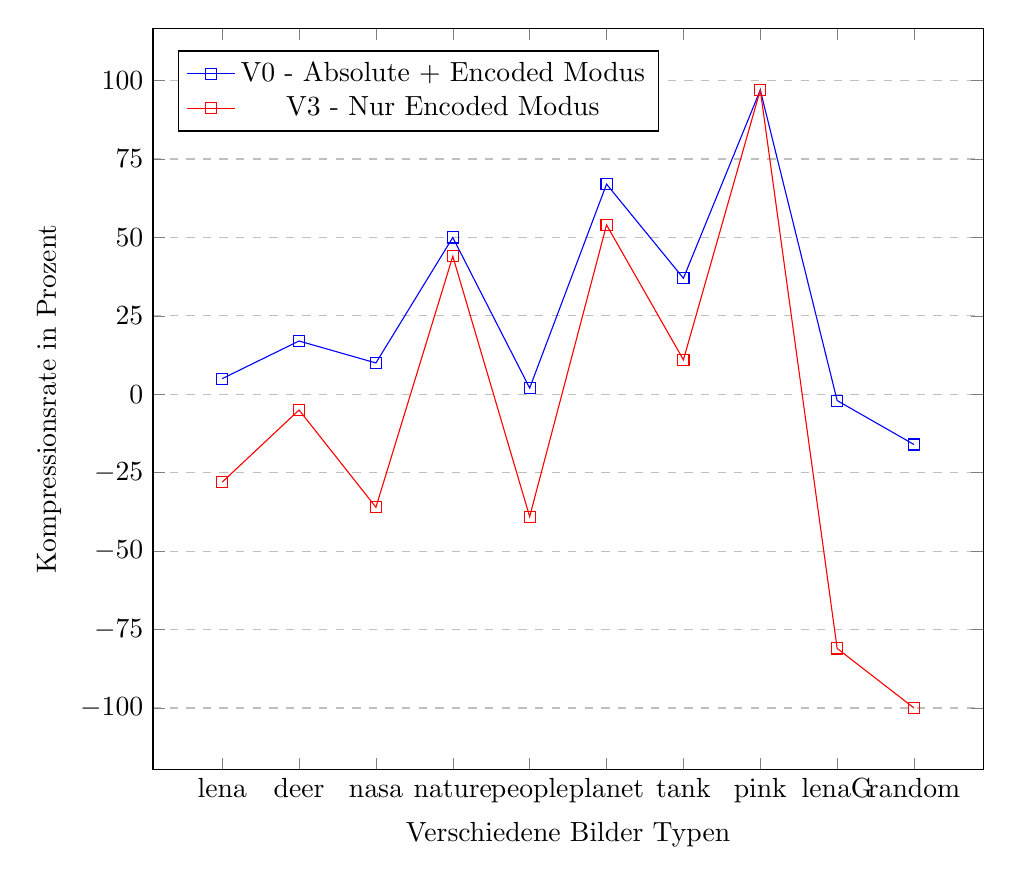
\begin{tikzpicture}
\begin{axis}[
    width  = 1*\textwidth,
    height = 11cm,
    xlabel={Verschiedene Bilder Typen},
    ylabel={Kompressionsrate in Prozent},
    % xmin=0, xmax=100,
    % ymin=0, ymax=120,
    xticklabel style={text height=1.5ex},
    symbolic x coords={lena, deer, nasa, nature, people, planet, tank, pink, lenaG, random},
    ytick={-100, -75, -50, -25, 0, 25, 50, 75, 100},
    legend pos=north west,
    ymajorgrids=true,
    grid style=dashed,
]

\addplot[
    color=blue,
    mark=square,
    ]
    coordinates {
    (lena,5)(deer,17)(nasa,10)(nature,50)(people,2)(planet,67)(tank,37)(pink,97)(lenaG, -2)(random,-16)
    };
    \addplot[
    color=red,
    mark=square,
    ]
    coordinates {
    (lena,-28)(deer,-5)(nasa,-36)(nature,44)(people,-39)(planet,54)(tank,11)(pink,97)(lenaG,-81)(random,-100)
    };
    \legend{V0 - Absolute + Encoded Modus, V3 - Nur Encoded Modus}
    
\end{axis}
\end{tikzpicture}
\caption{Kompressionsrate bei verschiedenen Bilder}
\label{fig:Kompressionsrate}
\end{figure}
\section{Zusammenfassung und Ausblick}
Die Lauflängenkodierung ermöglicht eine starke Verbesserung des Speicherverbrauchs, indem gleichfarbige Pixel zusammengefasst werden. Allerdings ist die Lauflängenkodierung nicht immer das effizienteste Komprimierungsverfahren, denn sie verkleinert nicht oder nur gering die Dateigröße von Bitmaps, die wenige gleichfarbige Pixel beinhalten. Für Bitmaps mit vielen gleichfarbigen Pixeln ist die Lauflängenkodierung immer noch ein effizientes Verfahren um die Dateigröße zu minimieren, so können im Average Case gute Kompressionsraten erreicht werden und im Best Case noch viel stärkere Kompressionsraten bis zu 64:1 (beim Schreiben von 255-Byte Blöcken).
\clearpage


% TODO: Fuegen Sie Ihre Quellen der Datei Ausarbeitung.bib hinzu
% Referenzieren Sie diese dann mit \cite{}.
% Beispiel: CR2 ist ein Register der x86-Architektur~\cite{intel2017man}.
\bibliographystyle{plain}
\bibliography{Ausarbeitung}{}

\end{document}

